
%(BEGIN_QUESTION)
% Copyright 2015, Tony R. Kuphaldt, released under the Creative Commons Attribution License (v 1.0)
% This means you may do almost anything with this work of mine, so long as you give me proper credit

\noindent
{\bf Lab Exercise -- introduction}

\vskip 5pt

Your task is to build, document, and troubleshoot a telemetry system consisting of an analog sensor connected to a data acquisition (DAQ) module, which then sends the data over Ethernet to a personal computer.  Temperature and pressure are suggested process variables to measure.  Electric current (measured using a shunt resistor or a current transformer) is another excellent process variable to measure, and this works well to introduce the specialized topic of electric power metering and protection.  In fact, setting up an electronic protective relay to sense AC current and initiate a breaker ``trip'' signal is an excellent alternative to using a generic DAQ.  Other process variables are open for consideration, though.

The following table of objectives show what you and your team must complete within the scheduled time for this lab exercise.  Note how some of these objectives are individual, while others are for the team as a whole:

\underbar{Objective completion table:}

% No blank lines allowed between lines of an \halign structure!
% I use comments (%) instead, so that TeX doesn't choke.

$$\vbox{\offinterlineskip
\halign{\strut
\vrule \quad\hfil # \ \hfil & 
\vrule \quad\hfil # \ \hfil & 
\vrule \quad\hfil # \ \hfil & 
\vrule \quad\hfil # \ \hfil & 
\vrule \quad\hfil # \ \hfil & 
\vrule \quad\hfil # \ \hfil & 
\vrule \quad\hfil # \ \hfil \vrule \cr
\noalign{\hrule}
%
% First row
{\bf Performance objective} & {\bf Grading} & {\bf 1} & {\bf 2} & {\bf 3} & {\bf 4} & {\bf Team} \cr
%
\noalign{\hrule}
%
% Another row
Team meeting and prototype sketch (do {\it first!}) & mastery & -- & -- & -- & -- & \cr
%
\noalign{\hrule}
%
% Another row
Circuit design challenge & mastery & & & & & -- -- -- -- \cr
%
\noalign{\hrule}
%
% Another row
Final documentation and system inspection & mastery & & & & & -- -- -- -- \cr
%
\noalign{\hrule}
%
% Another row
Demonstrate IP ``ping'' utility & mastery & -- & -- & -- & -- &  \cr
%
\noalign{\hrule}
%
% Another row
Demonstrate use of a ``knockout punch'' tool & mastery & -- & -- & -- & -- &  \cr
%
\noalign{\hrule}
%
% Another row
Accurate measurement of variable ($\pm$ 1\% of span) & mastery & -- & -- & -- & -- &  \cr
%
\noalign{\hrule}
%
% Another row
Data communicated via Ethernet & mastery & -- & -- & -- & -- &  \cr
%
\noalign{\hrule}
%
% Another row
Troubleshooting & mastery & & & & & -- -- -- -- \cr
%
\noalign{\hrule}
%
% Another row
Lab question: Instrument connections & proportional &  &  &  &  & -- -- -- -- \cr
%
\noalign{\hrule}
%
% Another row
Lab question: Commissioning & proportional &  &  &  &  & -- -- -- -- \cr
%
\noalign{\hrule}
%
% Another row
Lab question: Mental math & proportional &  &  &  &  & -- -- -- -- \cr
%
\noalign{\hrule}
%
% Another row
Lab question: Diagnostics & proportional &  &  &  &  & -- -- -- -- \cr
%
\noalign{\hrule}
%
% Another row
Decommission and lab clean-up & mastery & -- & -- & -- & -- &  \cr
%
\noalign{\hrule}
} % End of \halign 
}$$ % End of \vbox

The only ``proportional'' scoring in this activity are the lab questions, which are answered by each student individually.  A listing of potential lab questions are shown at the end of this worksheet question.  The lab questions are intended to guide your labwork as much as they are intended to measure your comprehension, and as such the instructor may ask these questions of your team day by day, rather than all at once (on a single day).

\vskip 10pt

{\bf It is essential that your team plans ahead what to accomplish each day.  A short (10 minute) team meeting at the beginning of each lab session is a good way to do this, reviewing what's already been done, what's left to do, and what assessments you should be ready for.  There is a lot of work involved with building, documenting, and troubleshooting these working instrument systems!}

As you and your team work on this system, you will invariably encounter problems.  You should always attempt to solve these problems as a team before requesting instructor assistance.  If you still require instructor assistance, write your team's color on the lab whiteboard with a brief description of what you need help on.  The instructor will meet with each team in order they appear on the whiteboard to address these problems.




\vfil \eject

\noindent
{\bf Lab Exercise -- team meeting, prototype sketch, and instrument selection}

\vskip 5pt

An important first step in completing this lab exercise is to {\bf meet with your instructor} as a team to discuss safety concerns, team performance, and specific roles for team members.  If you would like to emphasize exposure to certain equipment (e.g. use a particular type of control system, certain power tools), techniques (e.g. fabrication), or tasks to improve your skill set, this is the time to make requests of your team so that your learning during this project will be maximized.

\vskip 10pt

An absolutely essential step in completing this lab exercise is to work together as a team to {\bf sketch a prototype diagram} showing what you intend to build.  This usually takes the form of a simple electrical schematic and/or loop diagram showing all electrical connections between components, as well as any tubing or piping for fluids.  This prototype sketch need not be exhaustive in detail, but it does need to show enough detail for the instructor to determine if all components will be correctly connected for their safe function.

For example, if you intend to connect field devices to a PLC (Programmable Logic Controller), your prototype sketch must show how those devices will connect to typical input/output terminals on the PLC, where electrical power will be supplied, etc.  Prototype sketches need not show all intermediary connections between components, such as terminal blocks in junction boxes between the field device and the controller.

You should practice good problem-solving techniques when creating your prototype sketch, such as consulting equipment manuals for information on component functions and marking directions of electric current, voltage polarities, and identifying electrical sources/loads.  Use this task as an opportunity to strengthen your analytical skills!  Remember that you will be challenged in this program to do all of this on your own (during ``capstone'' assessments), so do not make the mistake of relying on your teammates to figure this out for you -- instead, treat this as a problem {\it you} must solve and compare your results with those of your teammates.

Your team's prototype sketch is so important that the instructor will demand you provide this plan before any construction on your team's working system begins.  {\it Any team found constructing their system without a verified plan will be ordered to cease construction and not resume until a prototype plan has been drafted and approved!}  Similarly, you should not deviate from the prototype design without instructor approval, to ensure nothing will be done to harm equipment by way of incorrect connections.  Each member on the team should have ready access to this plan (ideally possessing their own copy of the plan) throughout the construction process.  Prototype design sketching is a skill and a habit you should cultivate in school and take with you in your new career.

\vskip 10pt

Each lab team locker has its own data acquisition unit (DAQ), and other DAQ units are available from the instructor.  You will need to install software on a personal computer in order for that computer to gather analog data from the DAQ unit.

It is recommended that you test your DAQ before connecting it to any external circuitry.  For a simple test of an analog input, set your multimeter to ``Diode Test'' so that it outputs a small voltage, then connect your meter leads to one of the analog input channels on the DAQ: the software should register a small voltage on that channel, letting you know the DAQ is functioning.

\vskip 10pt

You will need to choose a suitable sensor to connect to one of the DAQ analog inputs.  For greatest accuracy, I recommend using a standard 4-20 mA loop-powered pressure or temperature transmitter, with a 250 ohm resistor connected to the DAQ so it can read a 1-5 volt signal:

$$\includegraphics[width=15.5cm]{i00350x01.eps}$$

\filbreak

You are also welcome to be more creative and build yourself a simpler analog sensing circuit such as this:

$$\includegraphics[width=15.5cm]{i00350x02.eps}$$

The challenge with a circuit such as this is that it will {\it not} output a signal that is linearly proportional to temperature like the loop-powered transmitter will.  In order to make this work, you will have to program a formula into the DAQ software to ``linearize'' the voltage signal into a proportional temperature value.  This will require extra work on your part to characterize the sensor, then develop a formula describing the signal voltage value as a function of the measured variable.  You may find a computer spreadsheet program to be helpful, plotting a curve of voltage versus sensor stimulus (e.g. temperature), then using the curve-fitting utility in the spreadsheet to develop an equation relating voltage to the measurement.

$$\includegraphics[width=15.5cm]{i00350x05.eps}$$

If you choose to build a system to measure AC current using a current transformer (CT, shown above), you will need to select a suitable shunt resistor to drop voltage generated by current output by the CT.  This is done by researching the ``burden'' rating of the CT, which will tell you how large that load resistor may be.  CTs act as current sources, and so ``want'' to drive a low-resistance load (e.g. an ammeter to measure the CT secondary current).  However, the DAQ needs to see a strong enough voltage drop across the shunt resistor to use a reasonable percentage of its range, in order to make good use of its resolution.  {\it If you build this circuit, you must be sure to do so in a way that the CT's secondary winding will never become open-circuited when load current goes through it!  Open-circuited current transformers are capable of generating dangerously high voltages!!!}

\vskip 10pt

{\bf Planning a functioning system should take no more than an hour if the team is working efficiently, and will save you hours of frustration (and possible component destruction!).}




\vfil \eject

\noindent
{\bf Lab Exercise -- circuit design challenge}

\vskip 5pt

Build a simple circuit using either a light sensor (photocell) or a temperature sensor (thermistor) connected to a fixed-value resistor and a battery such that a variable output voltage will be generated as the sensor is stimulated.  Your circuit must either make the voltmeter indication increase with increasing sensor stimulus (more voltage for more light or heat -- direct action), or do the exact opposite (reverse action), as specified by the instructor.  All electrical connections must be made using a terminal strip (no twisted wires, crimp splices, wire nuts, spring clips, or ``alligator'' clips permitted).  You will also need to demonstrate how to record and display the lowest and highest voltages output by this circuit using your digital multimeter's ``min/max'' recording function function.

This exercise tests your ability to properly identify the operating characteristics of a light or temperature sensor, properly size a resistor to form a voltage divider circuit with the sensor, properly connect a voltmeter into the circuit to achieve the specified response direction, properly use a DMM to capture minimum and maximum voltage values, and use a terminal strip to organize all electrical connections.

$$\includegraphics[width=15.5cm]{i00350x06.eps}$$

\vskip 10pt

The following components and materials will be available to you: assorted CdS {\bf photocells} and {\bf thermistors} ; an assortment of {\bf resistors} ; {\bf terminal strips} ; lengths of {\bf hook-up wire} ; {\bf battery clips} (holders).

\vskip 10pt

You will be expected to supply your own screwdrivers and digital multimeter (DMM) for assembling and testing the circuit at your desk.  The instructor will supply the battery(ies) to power your circuit when you are ready to see if it works.  Until that time, your circuit will remain unpowered.

\vskip 10pt

\noindent
{\bf Meter response} (instructor chooses): \hskip 20pt \underbar{\hskip 20pt} Direct \hskip 20pt \underbar{\hskip 20pt} Reverse

\vskip 10pt

\noindent
{\bf Captured value} (instructor chooses): \hskip 20pt \underbar{\hskip 20pt} $V_{minimum}$ \hskip 20pt \underbar{\hskip 20pt} $V_{maximum}$

\vskip 10pt

\noindent
{\bf Sensor type} (instructor chooses): \hskip 20pt \underbar{\hskip 20pt} Photocell \hskip 20pt \underbar{\hskip 20pt} Thermistor








\vfil \eject

\noindent
{\bf Lab Exercise -- building the system}

\vskip 5pt

The Instrumentation lab is set up to facilitate the construction of working instrument ``loops,'' with over a dozen junction boxes, pre-pulled signal cables, and ``racks'' set up with 2-inch vertical pipes for mounting instruments.  The only wires you should need to install to build a working system are those connecting the field instrument to the nearest junction box, and then small ``jumper'' cables connecting different pre-installed cables together within intermediate junction boxes.

After getting your prototype sketch approved by the instructor, you are cleared to begin building your system.  All wire connections should be made using terminal blocks.  No twisted or taped wire connections will be allowed.

\vskip 10pt

You will need to configure the DAQ software to ``scale'' the 1-5 VDC signal into an actual measurement of your process variable (e.g. temperature, pressure).  A requirement of this lab is that the DAQ software accurately register the process variable you are measuring, rather than merely displaying a voltage value from the sensor.

\vskip 10pt

The personal computer attached to the DAQ may be your own laptop, or one of the lab's computers.  Regardless of which computer you use, it needs to be connected to the lab's Ethernet network so that another computer in the lab may acquire the data from it.

\vskip 10pt

Your chosen system may require its own electrical enclosure to house the DAQ and/or other components, not already a part of the lab's permanently-installed loop system.  If you need to punch a hole in the side of a custom enclosure as part of your system, you must use a special tool called a {\it knockout punch} to make these holes (rather than use a hole saw on a drill).  The Greenlee company manufactures a line of knockout punches called the {\it Slug Buster}, which you may wish to research in preparing to use this tool.

\vskip 10pt

{\bf Common mistakes:}

\begin{itemize}
\item{} Starting to build the circuit before planning its construction on paper with a proposed circuit sketch.
\item{} Failing to heed signal voltage limits for the DAQ analog input channels.  {\it Be careful not to over-power the DAQ with signal voltages exceeding its measurement limits!}
\item{} Failing to tug on each and every wire where it terminates to ensure a mechanically sound connection.
\item{} Students working on portions of the system in isolation, not sharing with their teammates what they did and how.  It is important that the whole team learns all aspects of their system!
\end{itemize}

\vskip 10pt

{\bf Building a functioning system should take no more than one full lab session (3 hours) if all components are readily available and the team is working efficiently!}







\vfil \eject

\noindent
{\bf Lab Exercise -- advanced multimeter usage}

\vskip 5pt

Part of this lab exercise is learning how to use an incredibly powerful feature of your digital multimeter: its ability to capture and record minimum and maximum measurements.  On Fluke-brand multimeters, this mode is engaged by pressing a button labeled ``Min/Max''.  Once engaged, the meter will store in its memory the lowest, highest, and average values of that measurement from the time the mode is engaged until the time you read those captured values.

Some digital multimeters (DMMs) have even more advanced functionality, whereby they record multiple data points over time, more like a data recorder.  Additionally, other advanced features such as {\it high-speed Min/Max}, {\it high-resolution measurement}, and {\it low-pass filtering} are provided by Fluke-brand multimeters.  Take the time to try all of these measurement features while using your multimeter in this lab exercise.

\vskip 10pt

These functions are important when diagnosing intermittent faults in a system.  The multimeter's ability to capture and remember measurement values over long spans of time gives the technician the flexibility to set the multimeter as a recording device, leave to do other tasks, then return to see what the meter recorded during that span of time.

\vskip 10pt

It should be noted that your multimeter may not retain its automatic ranging capability when set to record data.  If your meter is like this and you engage this mode while the measurement value is low, the meter may respond with an ``overload'' indication should the measurement value exceed the range locked in at the time the record mode was engaged.  In this case, the you are advised to manually set the meter's measurement range before engaging the recording mode.

It should also be noted that some DMMs provide multiple sampling times for their record function.  In other words, your meter might provide a ``slow'' recording mode plus a ``fast'' recording mode.  The trade-off for faster sampling time is -- as always for DAQ hardware -- less measurement resolution.  In other words, you might not be able to record data as precisely as you would like in the fast speed.  Conversely, if you desire maximum resolution, you may have to settle for a slower sampling rate.

\vskip 10pt

{\bf Common mistakes:}

\begin{itemize}
\item{} Failing to consult the multimeter's instruction manual.
\item{} Failing to consult the multimeter's instruction manual.
\item{} Failing to consult the multimeter's instruction manual.
\item{} Note: {\it this repetition is not a typographical error.  I {\bf really} want you to consult the instruction manual that came with your multimeter!}
\end{itemize}






\vfil \eject

\noindent
{\bf Lab Exercise -- documenting the system}

\vskip 5pt

Each student must sketch their own {\it system diagram} for their team's data acquisition system.  This will not be an ISA-standard loop diagram, but rather a combination of schematic diagram (showing the sensor and DAQ connections) and block diagram (showing the computer Ethernet network complete with IP addresses).  Your diagram must be {\it comprehensive} and {\it detailed}, showing every wire connection, every cable, every terminal block, range points, network addresses, etc.  

An example system diagram is shown here:

$$\includegraphics[width=15.5cm]{i00350x03.eps}$$

When your entire team is finished drafting your individual diagrams, call the instructor to do an inspection of the system.  Here, the instructor will have students take turns going through the entire system, with the other students checking their diagrams for errors and omissions along the way.  During this time the instructor will also inspect the quality of the installation, identifying problems such as frayed wires, improperly crimped terminals, poor cable routing, missing labels, lack of wire duct covers, etc.  The team must correct all identified errors in order to receive credit for their system.  

After successfully passing the inspection, each team member needs to place their system diagram in the diagram holder located in the middle of the lab behind the main control panel.  When it comes time to troubleshoot another team's system, this is where you will go to find a diagram for that system!

\vskip 10pt

{\bf Common mistakes:}

\begin{itemize}
\item{} Forgetting to label all signal wires.
\item{} Forgetting to note all wire colors.
\item{} Forgetting to put your name on the diagram!
\item{} Basing your diagram off of a team-mate's diagram, rather than closely inspecting the system for yourself.
\item{} Not placing instruments in the correct orientation (field instruments on the left, control room instruments on the right).
\end{itemize}





\vfil \eject

\noindent
{\bf Lab Exercise -- DAQ signal scaling/linearization}

\vskip 5pt

Each team must configure the DAQ system to ensure it accurately measures and reports the measured variable.  The measurement accuracy will be checked by the instructor by applying random stimuli to the sensor while the team verifies the remote indication (on a computer connected through the network to the DAQ module).

If your system uses a loop-powered 4-20mA transmitter, the only DAQ configuration you will need to do is ``scale'' the DAQ so that it converts the linear 1-5 VDC signal into a linear representation of the measured variable.  However, you will need to rely on those teammates who have taken the INST24X courses to calibrate the transmitter so that it accurately outputs the 4-20 mA signal.

If your system reads a raw voltage signal from a resistive sensor in a bridge or other voltage-divider network, you will need to program the DAQ software to ``linearize'' the signal so that it will register the actual process variable and not just a plain signal voltage.  The following screenshot shows how a computer spreadsheet may be used to generate a linearizing equation from published sensor data:

$$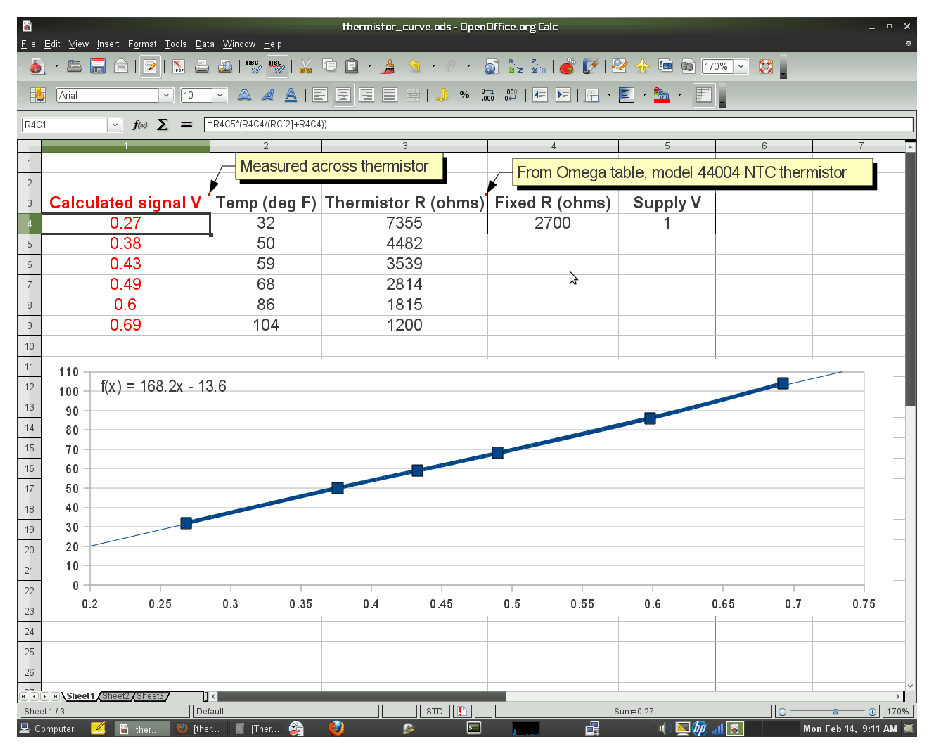
\includegraphics[width=15.5cm]{i00350x04.eps}$$

In this particular example, the sensor is a negative temperature coefficient (NTC) thermistor, model 44004, manufactured by Omega.  The formula entered into cells R4C1 through R9C1 calculates the voltage dropped across a fixed resistor (2700 $\Omega$) connected in series with the thermistor and powered by a 1 volt DC source, using the voltage divider equation ($V_R = V_{source} {R \over {R_{total}}}$).  The thermistor resistance values seen in column 3 were taken from an Omega-published table for the model 44004 thermistor.  A ``scatter'' plot graphs temperature as a function of voltage, and a ``trendline'' plotted by the spreadsheet program attempts to match the data points to a mathematical formula.  In this particular case, the fitted formula happens to be Temp = 168.2 * (Voltage) $-$ 13.6.  It is this formula you must enter into the DAQ software, so it knows how to translate the measured voltage signal into a temperature value.

\filbreak

If the sensor you choose does not have a data table describing its characteristics, you may generate your own by subjecting it to known stimuli and measuring its resistance at those known values.  Then, you may use a spreadsheet to plot the voltage response and derive an equation to fit the data.

Another huge advantage of using a computer spreadsheet to model the signal voltage as a function of temperature is that it allows you to ``experiment'' with different values of fixed resistance, to see the effect it has on linearity.  By entering a new fixed-resistor value into the spreadsheet, you may immediately see the effect that value change has on the curvature of the scatter plot, as well as the effect it has on the signal voltage strength.

\vskip 10pt

{\bf Common mistakes:}

\begin{itemize}
\item{} Choosing a poor-accuracy calibration standard (e.g. trying to calibrate your \$1500 precision Rosemount pressure transmitter to $\pm$ 0.1 PSI using a \$30 pressure gauge that only reads to the nearest 5 PSI!).
\item{} Improperly configuring the spreadsheet scatter plot to generate a fitted equation (e.g. having variables on wrong axes)
\end{itemize}

\vskip 10pt

{\bf Characterizing your sensor and scaling the DAQ software should take no more than one full lab session (3 hours) if the team is working efficiently!}






\vfil \eject

\noindent
{\bf Lab Exercise -- Ethernet data transfer}

\vskip 5pt

An essential part of this lab exercise is to have the acquired data transported over an Ethernet network.  Unless the DAQ software is quite sophisticated, this feature is not likely to be directly supported.  A suitable alternative is to have one computer acquiring data from the DAQ module, and use another computer to remotely view the display of the first computer.  This remote viewing may be done using ``Remote Desktop'' in Microsoft Windows operating systems, or by installing free remote-administration software such as {\tt RealVNC}.

Not only will remote access allow you to view the live DAQ data from another computer over the Ethernet network, but it also allows you do {\it operate} the DAQ computer remotely.  Knowing how to use remote-viewing software, therefore, is a very useful skill.

\vskip 10pt

Another Ethernet-related objective in this lab exercise is using the {\tt ping} utility to test for network connections.  When two personal computers have been successfully connected to a common Ethernet network, you should be able to ``ping'' one computer from the other by invoking the {\tt ping} utility with the IP address of the destination computer as an argument to the {\tt ping} command.  You may run the {\tt ping} command from a command-line window on a Microsoft Windows operating system.  More detailed instructions on the use of {\tt ping} may be found in your {\it Lessons In Industrial Instrumentation} textbook.

A successful ``ping'' from one computer to another is a {\it necessary} condition for remote viewing of that computer's display, but it is not a {\it sufficient} condition.  That is to say, although a computer that refuses to ``ping'' is definitely not ready to be logged into remotely, a computer that does ``ping'' without trouble may not necessarily be ready for remote login.  Getting a successful ``ping'' from a computer is merely the first step in establishing full communication with it.

\vskip 10pt

If a ``ping'' attempt proves unsuccessful, it means something is inhibiting communication between that device and the computer you're using to issue the ping.  A good test to do in this circumstance is try ``pinging'' other devices on that same network.  Any successful ping attempts will definitively prove OSI layers 1, 2, and 3 are all functional between those two points, since ``ping'' requires those three layers to function.  Once you know which portion(s) of the network are functional, you may narrow the field of fault possibilities.

\vskip 10pt

Network functions above OSI layer 3 (e.g. ``firewall'' software running on personal computers) are capable of inhibiting communication between devices on the lab's Ethernet network, including ``ping'' messages.  If you decide to connect your own personal computer (laptop) to the lab's Ethernet network, you may find it easier to temporarily disable all security features on your personal computer to enable free and open communication between your computer and all other devices on the network.  Just be sure to re-enable the security features when you are done, so your computer will not be unprotected the next time you connect to the Internet!







\vfil \eject

\noindent
{\bf Lab Exercise -- troubleshooting}

\vskip 5pt

The most challenging aspect of this lab exercise is {\it troubleshooting}, where you demonstrate your ability to logically isolate a problem in the system.  All troubleshooting is done on an individual basis (no team credit!), and must be done {\it on a system you did not help build}, so that you must rely on loop diagrams to find your way around the system instead of from your own memory of building it.

Each student is given a limited amount of time to identify both the general location and nature of the fault, logically justifying all diagnostic steps taken.  All troubleshooting activities will take place under direct instructor supervision to ensure students are working independently and efficiently. 

Failure to correctly identify both the general location and nature of the fault within the allotted time, and/or failing to demonstrate rational diagnostic procedure to the supervising instructor will disqualify the effort, in which case the student must re-try with a different fault.  Multiple re-tries are permitted with no reduction in grade.

A standard multimeter is the only test equipment allowed during the time limit.  No diagnostic circuit breaks are allowed except by instructor permission, and then only after correctly explaining what trouble this could cause in a real system.  

The instructor will review each troubleshooting effort after completion, highlighting good and bad points for the purpose of learning.  Troubleshooting is a skill born of practice and failure, so do not be disappointed in yourself if you must make multiple attempts to pass!  One of the important life-lessons embedded in this activity is how to deal with failure, because it {\it will} eventually happen to you on the job!  There is no dishonor in failing to properly diagnose a fault after doing your level best.  The only dishonor is in taking shortcuts or in giving up.

\vskip 10pt

{\bf Common mistakes:}

\begin{itemize}
\item{} Neglecting to take measurements with your multimeter.
\item{} Neglecting to check other measurements in the system (e.g. pressure gauge readings).
\item{} Incorrectly interpreting the diagram (e.g. thinking you're at the wrong place in the system when taking measurements).
\item{} Incorrect multimeter usage (e.g. AC rather than DC, wrong range, wrong test lead placement).  This is especially true when a student comes to lab unprepared and must borrow someone else's meter that is different from theirs!
\end{itemize}

\vskip 10pt

{\bf Remember that the purpose of the troubleshooting exercise is to foster and assess your ability to intelligently diagnose a complex system.  Finding the fault by luck, or by trial-and-error inspection, is not a successful demonstration of skill.  The only thing that counts as competence is your demonstrated ability to logically analyze and isolate the problem, correctly explaining all your steps!}

\vskip 10pt

{\bf Troubleshooting takes a lot of lab time, usually at least two 3-hour lab sessions for everyone in a full class to successfully pass.  Be sure your team budgets for this amount of time as you plan your work, and also be sure to take advantage of your freedom to observe others as they troubleshoot, to better learn this art.}




\vfil \eject

\noindent
{\bf Lab questions}

\vskip 5pt

\begin{itemize}
\item{} {\bf Instrument connections}
\item{} Determine correct wire connections between a DAQ module and an electrical sensor, based on diagrams of instruments with terminals labeled
\item{} Correctly determine all electrical sources and loads, as well as all voltage polarities and current directions in a DAQ/sensor circuit, based on diagrams of instruments with terminals labeled
\end{itemize}

\filbreak

\begin{itemize}
\item{} {\bf Commissioning and Documentation}
\item{} Explain the operating principle of the sensor used in your system
\item{} Explain the difference between a {\it single-ended} input channel and a {\it differential} input channel on an analog DAQ module
\item{} Describe the use of some of the advanced functions of your multimeter {\it besides} record (``Min/Max'') mode
\item{} Explain why power and signal wiring should not be run together in conduit or in a panel
\item{} Explain why it is necessary to use a {\it bushing} to protect electrical wires that enter and exit an electrical enclosure through a hole in the side of that enclosure
\end{itemize}

\filbreak

\begin{itemize}
\item{} {\bf Mental math} (no calculator allowed!)
\item{} Determine allowable calibration error of instrument (e.g. +/- 0.5\% for an instrument ranged 200 to 500 degrees)
\item{} Convert 1-5 V signal into a percentage of span (e.g. 3.5 V = \underbar{\hskip 20pt}\%)
\item{} Convert percentage of span into a 1-5 V signal value (e.g. 70\% = \underbar{\hskip 20pt} V)
\item{} Calculate resolution of ADC given number of bits and input signal range
\end{itemize}

\filbreak

\begin{itemize}
\item{} {\bf Diagnostics}
\item{} Explain how to distinguish an ``open'' cable fault from a ``shorted'' cable fault using only a voltmeter (no current or resistance measurement, but assuming you are able to break the circuit to perform the test)
\item{} Determine whether or not a given diagnostic test will provide useful information, given a set of symptoms exhibited by a failed system
\item{} Identify at least two plausible faults given the results of a diagnostic test and a set of symptoms exhibited by a failed system
\item{} Propose a diagnostic test for troubleshooting a failed system and then explain the meanings of two different test results
\end{itemize}



\vfil \eject

\noindent
{\bf Lab Exercise -- decommissioning and clean-up}

\vskip 5pt

The final step of this lab exercise is to decommission your team's entire system and re-stock certain components back to their proper storage locations, the purpose of which being to prepare the lab for the next lab exercise.  Remove your system documentation (e.g. loop diagram) from the common holding area, either discarding it or keeping it for your own records.  Also, remove instrument tag labels (e.g. FT-101) from instruments and from cables.  Perform general clean-up of your lab space, disposing of all trash, placing all tools back in their proper storage locations, sweeping up bits of wire off the floor and out of junction boxes, etc.

\vskip 10pt

\indent
{\bf Leave the following components in place, mounted on the racks:}

\begin{itemize}
\item{} Large control valves and positioners
\item{} I/P transducers
\item{} Large electric motors
\item{} Large variable-frequency drive (VFD) units
\item{} Cables inside conduit interconnecting junction boxes together
\item{} Pipe and tube fittings (do not unscrew pipe threads)
\item{} Supply air pressure regulators
\end{itemize}

\vskip 10pt

\indent
{\bf Return the following components to their proper storage locations:}

\begin{itemize}
\item{} Sensing elements (e.g. thermocouples, pH probes, etc.)
\item{} Process transmitters
\item{} ``Jumper'' cables used to connect terminal blocks within a single junction box
\item{} Plastic tubing and tube fittings (disconnect compression-style tube fittings)
\item{} Power cables and extension cords
\item{} Adjustment (loading station) air pressure regulators
\end{itemize}

\vskip 10pt

Finally, you shall return any control system components to their original (factory default) configurations.  This includes controller PID settings, function block programs, input signal ranges, etc.


\underbar{file i00350}
%(END_QUESTION)





%(BEGIN_ANSWER)

There exist some inexpensive data acquisition modules on the market for personal computers, including some with USB interfaces (and most with RS-232 serial interfaces).  If all you have is a serial-interface module and a USB-only computer (as most laptop computers are!), you may use a USB-to-serial adapter to connect the serial DAQ device to the personal computer.  Within Microsoft Windows, you may force the operating system to recognize the USB adapter as an old-style COM 1 or COM 2 RS-232 serial device, at which time the DAQ software should ``talk'' through the adapter to the DAQ module seamlessly.

%(END_ANSWER)





%(BEGIN_NOTES)

\noindent
{\bf Diagrams / inspections:}

I strongly recommend checking off students' diagrams while you inspect their system (checking for secure wiring, proper tubing, good conduit installation, etc.) with them.  Have all team members take you on a ``tour'' of their completed system, with each team member explaining a different portion of the system you select while using their own diagram as a guide.  While a student is explaining their section of the system, you can check the other students' diagrams for accuracy.  This not only saves time by consolidating the tasks of system inspection and diagram verification, but it also ensures students can actually relate their diagrams to the system they have built and articulate that understanding to you.

\vskip 10pt

\goodbreak

\noindent
{\bf Troubleshooting fault ideas:}

\begin{itemize}
\goodbreak
\item{} Strip wire at terminal, then insert insulated wire end under terminal and tighten (open wire fault)
\item{} Cut signal cable somewhere in mid-conduit (open wire fault)
\item{} Unplug Ethernet cable
\item{} Change IP address or network mask of one computer
\item{} Wire instrument cable conductors backward (construction fault)
\item{} Configure transmitter for excessive damping (slow response fault)
\item{} Configure indicator/controller for excessive damping (slow response fault)
\item{} Miscalibrate transmitter and/or indicator/controller (inaccuracy fault)
\item{} Plug tube connections using portion of foam earplug stuffed into tube fitting (slow response fault)
\item{} Mis-configure linear characterization of transmitter and/or DAQ (nonlinearity fault)
\item{} Mis-configure function block inside DAQ (e.g. change limit values to simulate signal stuck either low or high; disconnect signal line between two blocks)
\item{} Connect 2.2 k resistor in parallel with 4-20 mA transmitter to simulate partial short in wiring (inaccuracy fault)
\item{} Exchange 250 ohm resistor for a different resistor that looks the same but has the wrong value (inaccuracy fault) 
\item{} Give students wrong diagram (documentation fault)
\end{itemize}















\vfil \eject

\noindent
{\bf Lab questions}

\vskip 20pt

\item{$(1)$} Connect the transmitter to register pressure on channel 3 on the DAQ:

$$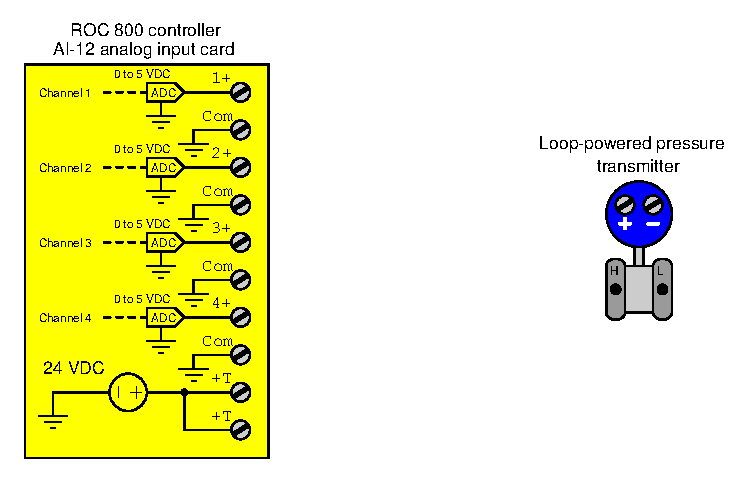
\includegraphics[width=15.5cm]{i00350x07.eps}$$

\vskip 20pt

\item{$(2)$} Explain the difference between {\it single-ended} and {\it differential} inputs on an analog DAQ module.

\vskip 20pt

\item{$(3)$} Determine the allowable calibration error of a pressure transmitter with a range of 0 to 300 PSI and a calibration tolerance of $\pm$ 0.5\%.  Express your answer in units of PSI.

\vskip 20pt

\item{$(4)$} PC number 3 (IP address 192.168.0.2) cannot connect to the internet.  Identify one diagnosic test you could perform on this system, then describe {\it two (different) possible results} of that test and explain what each result would mean in terms of locating the fault:

$$\includegraphics[width=15.5cm]{i00350x09.eps}$$

















\vfil \eject

\noindent
{\bf Lab questions}

\vskip 20pt

\item{$(1)$} Connect the transmitter to register pressure on channel 2 on the DAQ:

$$\includegraphics[width=15.5cm]{i00350x08.eps}$$

\vskip 20pt

\item{$(2)$} Identify at least one of the advanced functions offered by your multimeter {\it besides} record (``Min/Max'') mode.

\vskip 20pt

\item{$(3)$} Convert a 2.5 volt signal (in a 1-5 volt range) into a value expressed in {\it percent}.

\vskip 20pt

\item{$(4)$} PC number 5 (IP address 192.168.0.29) cannot connect to PC number 1 (IP address 192.168.0.35).  Identify one diagnosic test you could perform on this system, then describe {\it two (different) possible results} of that test and explain what each result would mean in terms of locating the fault:

$$\includegraphics[width=15.5cm]{i00350x09.eps}$$


%INDEX% Lab exercise, data acquisition and Ethernet networking

%(END_NOTES)


